% File hicss51.tex
%%
%% Based on the style files for ACL 2015 by 
%% car@ir.hit.edu.cn, gdzhou@suda.edu.cn


\documentclass[10pt]{article}
\usepackage[letterpaper]{geometry}
\usepackage{hicss51}
\usepackage{times}
\usepackage[none]{hyphenat}
\usepackage{url}
\usepackage{latexsym}
%\usepackage{minted}
\usepackage{indentfirst}
\usepackage{graphicx}
%\graphicspath{{images/}}
\usepackage{wrapfig}
\usepackage{todonotes}
\usepackage{hyperref}
\usepackage[utf8]{inputenc}
\newcommand{\sansserifformat}[1]{\fontfamily{cmss}{ #1}}%

%\setlength\titlebox{5cm}


% You can expand the titlebox if you need extra space
% to show all the authors. Please do not make the title box
% smaller than 5cm (the original size).



\title{Open Source Intelligence - Development of a Trend Radar utilizing a Systematic Literature Review}

\author{Franz Kayser \\
  ESG \\
  {\underline{ franz.kayser@esg.de}} \\\And
  Thomas Mayer \\
  ESG  \\
  {\underline{ thomas3.mayer@esg.de} }\\\And 
  Michael Bücker \\
  FH Münster -- University of Applied Sciences\\
  {\underline{michael.buecker@fh-muenster.de}} \\}

\date{}

\begin{document}
\maketitle
\begin{abstract}
    Open Source Intelligence (OSINT) is currently experiencing an intensive discourse,
    heightened since the Russian invasion of Ukraine. However, despite numerous attempts
    at standardized definitions, the intelligence discipline remains ambiguous. This paper
    introduces a practice-validated OSINT trend radar, categorizing technologies by maturity,
    intelligence cycle phase, and use case. Serving as a profound knowledge base and tool for
    identifying research gaps, the radar emerges from a structured design process. Sixty
    studies underwent categorization and validation through expert interviews,
    revealing the absence of a comprehensive, autonomous third-generation OSINT
    system in Germany. Technological gaps, especially in the planning and direction and
    dissemination and integration phases, are evident. Although intelligent support
    technologies were identified, practical implementation lags behind theory. The human
    factor therefore remains central to the OSINT process. Future research should thus
    prioritize developing applications for underserved phases, probing reasons for limited
    widespread implementation of proven applications, with emphasis on legal, ethical,
    political, and social parameters.
\end{abstract}

\section{Introduction} \label{sec:introduction}

OSINT, the process of gathering intelligence from publicly available data, has gained considerable attention, particularly since
the 2022 Russian invasion of Ukraine \cite{DosPassos.2017}. Real-time analysis of social media has proven pivotal in revealing
valuable insights \cite{Hatfield.2023, SmithBoyle.24.07.2023}. Despite numerous attempts to define OSINT
\cite{Hwang.2022, PastorGalindo.2020, Yogish.2021}, controversy persists, influenced by ongoing advancements in computer and
data sciences that continuously enhance collection and analysis capabilities \cite{Ghioni.2023, Williams.2018}. The
proliferation of open communication channels has led to an overwhelming "information explosion"
\cite{DosPassos.2017, Hwang.2022, Yogish.2021}, with formerly restricted data sources now publicly accessible
\cite{Hwang.2022, Williams.2018}, fundamentally reshaping intelligence paradigms \cite{Dokman.2020}.
Despite this heightened interest, fundamental scientific literature in the field remains limited \cite{HerreraCubides.2020},
failing to keep pace with rapid developments \cite{Ghioni.2023, Williams.2018}. Key questions regarding the existence of
autonomous third-generation OSINT systems \cite{PastorGalindo.2019, PastorGalindo.2020} remain unanswered
\cite{Ghioni.2023, PastorGalindo.2020, Yogish.2021}, with a disproportionate focus on cybersecurity within existing
studies \cite{Hwang.2022, PastorGalindo.2019, Yogish.2021}. Consequently, significant OSINT use cases remain unexplored
\cite{AlKilani.2021, Dokman.2020, Ghioni.2023}, lacking qualitative field research to bridge theoretical concepts with
practical implementation \cite{HerreraCubides.2020, PastorGalindo.2019}. This study is guided by the overarching research
question: \textit{How can the current trends in OSINT, focusing on technologies and their characteristics, maturity levels,
    and use cases, be presented in a trend radar and validated by experts within the security sector?}

In response to this question,
the paper investigates current OSINT trends, adopting the Design Science Research Model (DSRM) \cite{Peffers.2007}.
The methodology involves a systematic literature review \cite{Webster.2002} to analyze and classify relevant OSINT literature.
Subsequently, OSINT technologies and their characteristics will be visualized in a trend radar, validated through systematizing
interviews with security sector experts \cite{Bogner.2014}, and evaluated using qualitative content analysis \cite{Billings.1997}.


\section{Theoretical Background} \label{sec:theoreticalbackground}

The domain of OSINT is continuously expanding due to the ongoing improvements of
collecting and analysis possibilities \cite{Ghioni.2023, Williams.2018}. In
addition, the new means and methods of communication associated with advances in information
and communication technology have turned OSINT into a complex discipline
\cite{Benes.2013, Williams.2018}.

\subsection{Open Source Intelligence (OSINT) and its Components}

One of the earliest and still frequently referenced definitions \cite{DosPassos.2017}
was published by NATO in 2001. OSINT according to this definition is information that has been
deliberately discovered, discriminated, distilled, and disseminated to a select audience,
[...], in order to address a specific question. OSINT, [...] thus applies the proven
process of intelligence to the broad diversity of open sources [...] and creates
intelligence \cite{NorthAtlanticTreatyOrganization.2001}. However, today the discipline is no longer seen as a purely governmental
matter. Private research institutions and organizations \cite{Bohm.2021,Mercado.2005} are
also massively driving the development of such systems
\cite{Dokman.2020, Ghioni.2023}. The focus is thereby shifting to
developing OSINT into a robust, autonomous solution (referred to as third-generation) \cite{PastorGalindo.2019}.

\subsection{Intelligence and Intelligence Cycle}

The core task of OSINT is to generate intelligence
in terms of a profound basis for decision-making
\cite{Breakspear.2013,NorthAtlanticTreatyOrganization.2001}. The generation process of such an intelligence product
is also referred to as the intelligence cycle \cite{CentralIntelligenceAgency.1987}.
It represents the central element of every intelligence discipline \cite{Reuser.2017}. The link between the phases is that
the result of the preceding phase serves as input for the subsequent phase
\cite{JointChiefsofStaffU.S.Army.2013}. Furthermore, the individual phases are also continuously
iterated due to the fulfillment of previous requirements and new demands\cite{Gibson.2016}.
Today, to represent external influences or the
assignment of responsibilities \cite{Lowenthal.2020,Phythian.2013}, numerous
variations can be found \cite{Reuser.2017}. The
Intelligence Cycle should therefore be seen less as a guideline and more as an informal
coordination element\cite{Hwang.2022}.
In 2013, the JCS segmented the cycle into 6 phases \cite{JointChiefsofStaffU.S.Army.2013} (see figure \ref{fig: intelligence cycle}).

\begin{figure}[h]
    \centering
    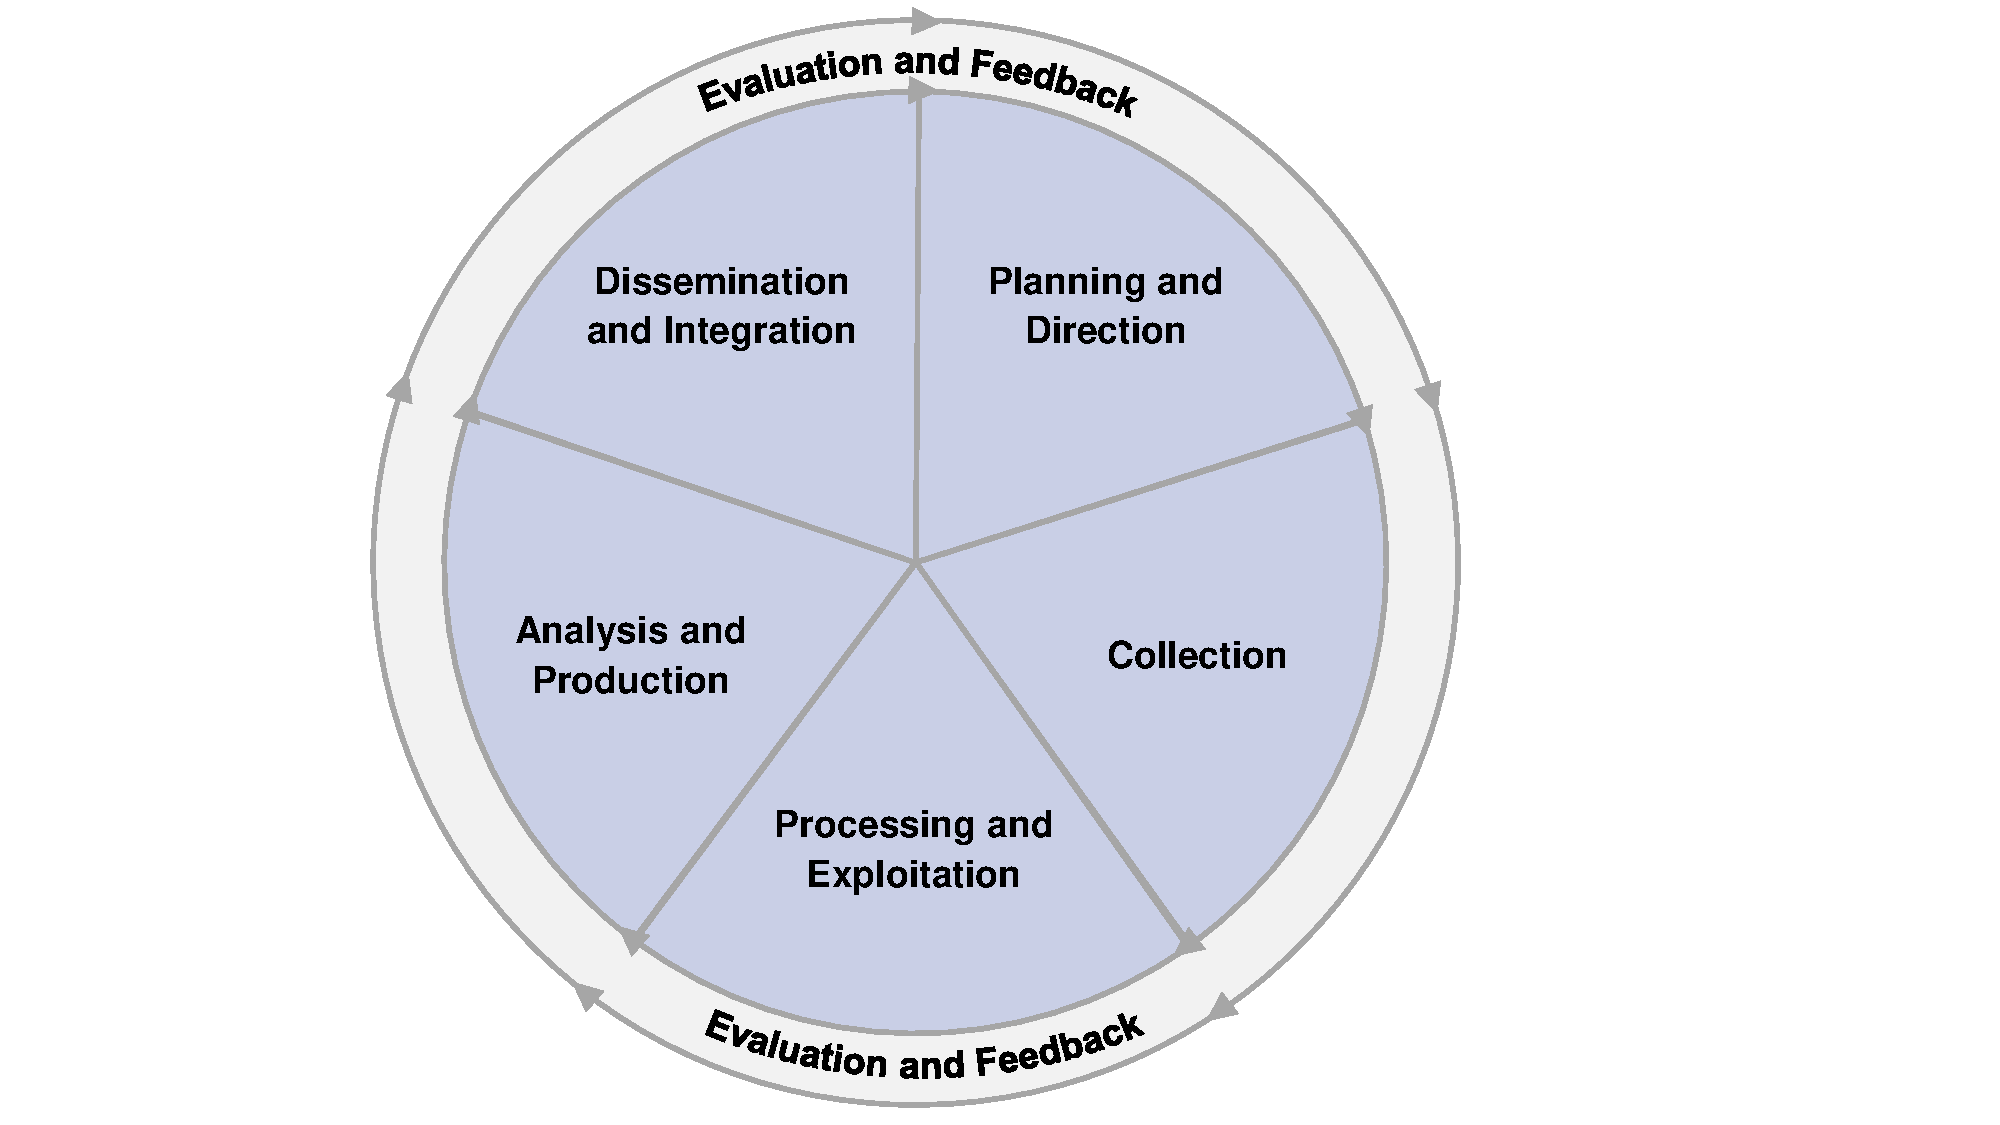
\includegraphics[clip,width=0.8\linewidth]{PDF/images/crop_Intelligence Cycle}
    \caption{Intelligence Cycle, according to \cite{JointChiefsofStaffU.S.Army.2013}}
    \label{fig: intelligence cycle}
\end{figure}

The planning and direction phase combines the identification, definition, prioritization and monitoring
of the requirements for the cycle\cite{JointChiefsofStaffU.S.Army.2013}.
The collection phase refers to the gathering of raw data \cite{CentralIntelligenceAgency.1987}.
The core of this phase consists of the iterative repetition of research
\cite{NorthAtlanticTreatyOrganization.2001} to make the query more precise with each run
\cite{PastorGalindo.2020}. The processing and utilization phase involves condensing
these data volumes into action-relevant information
\cite{JointChiefsofStaffU.S.Army.2013}.
Analysis and production refers to the synthesis of the information obtained into a
user-oriented, timely and accurate intelligence product
\cite{Hwang.2022, NorthAtlanticTreatyOrganization.2001}.
The final phase consists of handing over the finished product to the "customer" in a
usable form \cite{CentralIntelligenceAgency.2023, Williams.2018}.
Evaluation and feedback are not to be regarded as individual phases
but take place continuously throughout the entire cycle. The aim is to achieve progressive optimization
\cite{JointChiefsofStaffU.S.Army.2013, NorthAtlanticTreatyOrganization.2001}.

\subsection{Previous Studies}

Eight previous, publicly accessible literature reviews can be identified
concerning OSINT. In 2017, Dos Passos \cite{DosPassos.2017} showed how big data and data science can
make the decision-making process more useful and effective. Pastor-Galindo et al. then described
the current state of OSINT in 2019 \cite{PastorGalindo.2019} and 2020 \cite{PastorGalindo.2020}
focusing on services and techniques to improve cybersecurity. Moreover, they are responsible
for the first and only rudimentary mapping of OSINT trends. They observed that OSINT is used in
social opinion and sentiment analysis, cybercrime and organized crime, as well as cybersecurity and cyberdefence.
Two further literature reviews were published in 2020. García Lozano et al. \cite{GarciaLozano.2020} identified
methods for computer-assisted veracity assessment of public information.
Herrera-Cubides et al. \cite{HerreraCubides.2020} investigated how the production of
research and educational materials has developed. They concluded that
the number of OSINT publications is lower compared to other trending topics. In 2021,
Yogish and Krishna \cite{Yogish.2021} explored the state of implementation and use of
Artificial Intelligence (AI) technologies in the context of cybersecurity. The result of this
study showed that Machine Learning (ML), pattern recognition and Natural Language Processing
(NLP) can simplify OSINT given increasing data volumes. In the following year, Hwang et al.
\cite{Hwang.2022} investigated security threats and cybercriminality in the context of OSINT misuse.
In 2023, Ghioni et al. \cite{Ghioni.2023} then examined the political, ethical, legal and social implications of
OSINT in conjunction with AI. They discovered that there is still no framework
for addressing these. They also found that third-generation OSINT is still in its early
stages and that human components cannot yet be replaced.


\section{Research Methodology}

The structure of the study is based on the iterative Design Science Research Model (DSRM) \cite{Peffers.2007}. It is a theory-based
research paradigm for developing an explicitly applicable solution, in the form of an innovative artifact,
\cite{vomBrocke.2020b}, solving a (practical) problem \cite{Peffers.2007}. The model is therefore ideally suited to
create the trend radar. It consists of six successive activities \cite{Peffers.2007}:

\begin{enumerate}
    \item Problem identification and motivation
    \item Objectives of the solution
    \item Design and development
    \item Demonstration
    \item Evaluation
    \item Communication
\end{enumerate}

We will discuss steps 2-5 indetail, while the first step (problem identification and motivation) is summarized in section \ref{sec:introduction} and results of step 6 (communication) are described in sections \ref{sec:results} and \ref{sec:discussion}. Following \cite{Sonnenberg.2012}, steps 1-4 were continuously evaluated during the study.

%\begin{figure*}[thb]
%    \centering
%    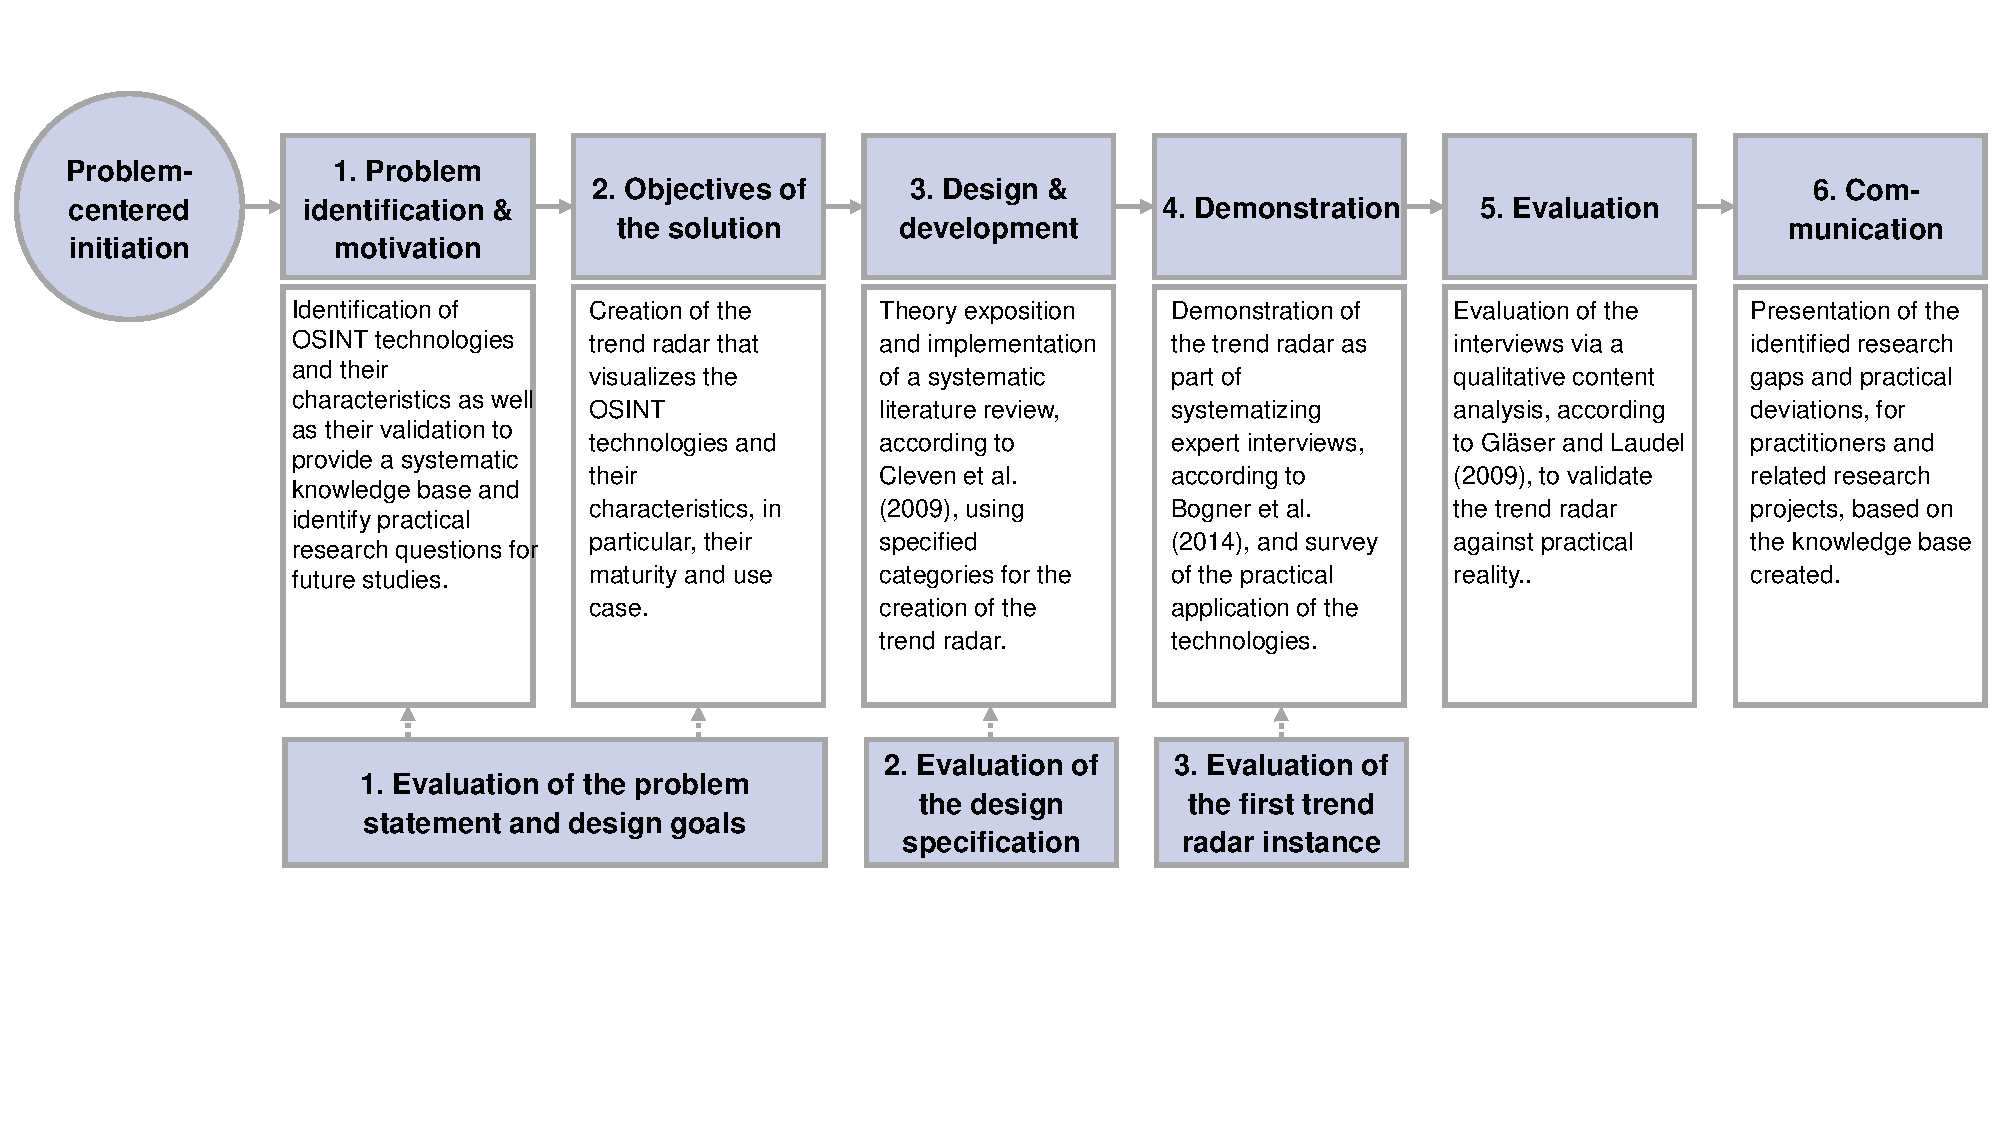
\includegraphics[width=\textwidth]{PDF/images/crop_DSRM}
%    \caption{Design Science Research Model (DSRM)}
%    \label{fig: DSRM}
%\end{figure*}

\subsection{Design Objectives of the Solution}

The design objectives of the solution are divided into content-related objectives (CO) and formal objectives (FO).

\textbf{Content-related objectives (CO)}
\begin{itemize}
    \item[CO1] The trend radar must follow a procedural structure that reflects the process of generating intelligence. This will allow a structured mapping of the identified technologies according to their use. In doing so, any research gaps that become apparent can be directly assigned to the respective phase. It will thus be possible to verify if a third-generation OSINT system exists.
    \item[CO2] The key characteristics, in particular the maturity level of the technologies and their use cases, must be taken into account. The maturity level of the technologies makes it possible to determine the respective research status. Through the use cases, the research directions can be revealed.
\end{itemize}

\textbf{Formal objectives (FO)}
\begin{itemize}
    \item[FO1] The trend radar must follow a simple structure to enable the immediate identification of research gaps. In addition, the radar should have a high degree of standardization to be transferable to other intelligence gathering disciplines in later studies.
    \item[FO2] The trend radar should be continuously expandable to capture the high field dynamics.
\end{itemize}


\subsection{Evaluation of the Problem Statement and Design Objectives}

In Section \ref{sec:theoreticalbackground}, we define key concepts foundational to our research, focusing particularly on the intelligence cycle. This cycle is crucial as it forms the theoretical basis for the development of our trend radar tool, which we assess for its suitability within the OSINT framework. Additionally, our review of prior studies exposes a notable gap in comprehensive research on OSINT, highlighting the importance and relevance of our inquiry.


\subsection{Design and Development}
In the third activity of the DSRM, the creation of the artifact involves conducting a systematic literature review, as delineated by \cite{Cleven.2009}. Utilizing Cooper's taxonomy \cite{Cooper.1988} for scoping the literature review, we established classification categories to create concept matrices for a structured analysis of the literature \cite{Webster.2002}.

To ensure a standardized approach across the intelligence cycle, general categories were defined corresponding to each phase, with the evaluation and feedback phases integrated due to their iterative nature. For the collection phase, the following six categories were developed:
\begin{itemize}
    \item \textbf{Use case:} Application areas of the technologies.
    \item \textbf{Data:} Composition and types of data foundations, including data format and source.
    \item \textbf{Process:} Degree of automation in the technologies, categorized into manual, semi-automated, automated, and fully automated/autonomous \cite{Duncheon.2002, Billings.1997, Endsley.1999}.
    \item \textbf{Technology:} Material and immaterial means used for managing information \cite{Bleck.2004}.
    \item \textbf{Technology Complexity:} Assessed through subcategories of Volume, Variety, and Velocity \cite{Elgendy.2014, Singh.2012}.
    \item \textbf{Maturity Level:} Based on the phases of innovation, prototype, and market establishment \cite{Stich.2022}.
\end{itemize}

Similar categories were adapted for other phases of the intelligence cycle, with complexity measured via the analytics spectrum: descriptive, diagnostic, predictive, and prescriptive \cite{Delen.2013}.

The literature search, executed using a broad search string to maximize retrieval, was limited to publications from 2020 to 2023 to reflect recent advancements. A total of 60 studies were analyzed using the SQR3 method \cite{Robinson.1970} and categorized into a meticulously structured Excel spreadsheet for each phase of the intelligence cycle (Fig. \ref{fig:LiteratureReview}).

\begin{figure}[t]
    \centering
    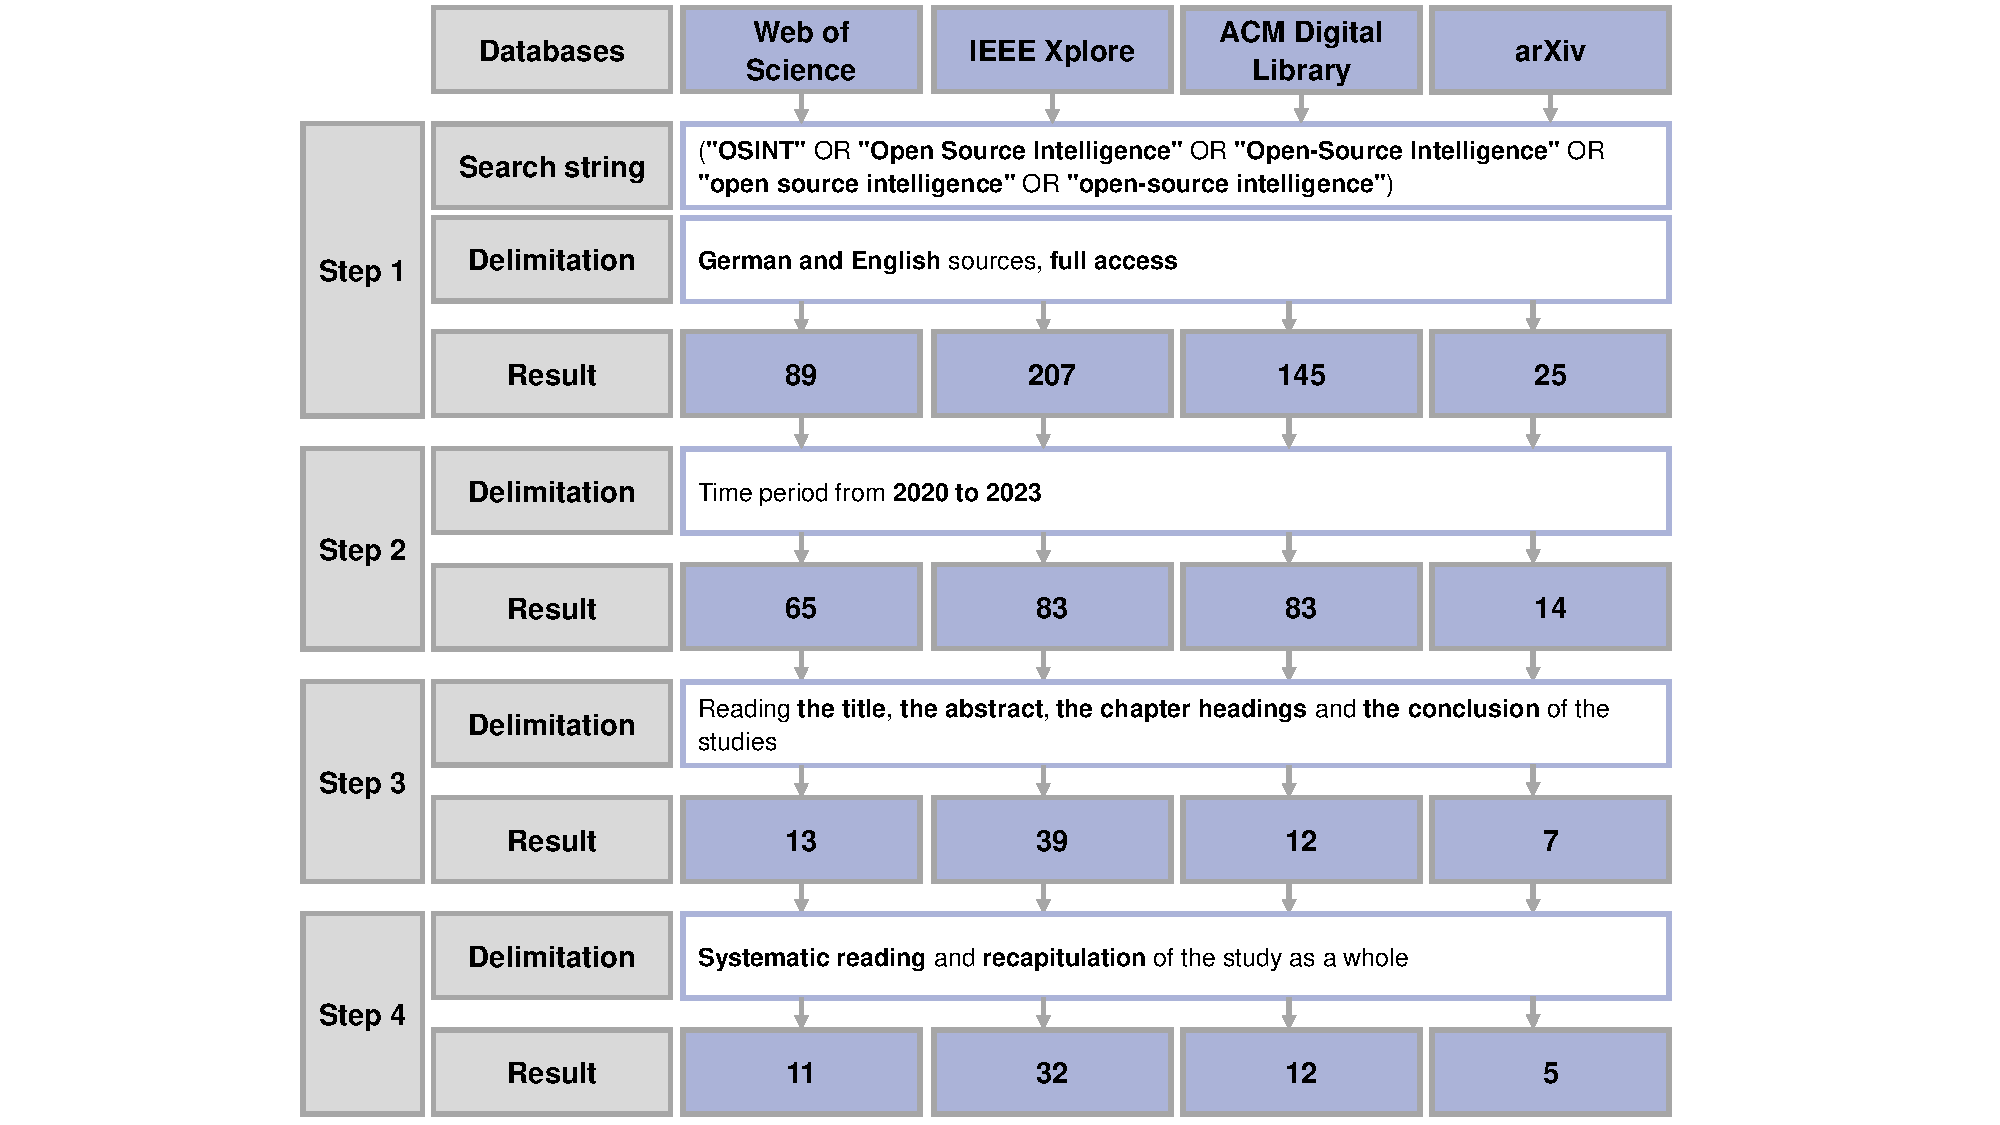
\includegraphics[width=0.4\textwidth]{PDF/images/crop_Kategorisierungskriterien und Literraturreviewaufbau}
    \caption{Literature review setup and categorization criteria}
    \label{fig:LiteratureReview}
\end{figure}

Each technology was then categorized and analyzed for interrelationships within the OSINT framework. Verification of categorization was conducted using a Python script, which scanned the included papers for predefined keywords. The validated categories and relationships informed the development of the trend radar based on the verified concept matrices.


\subsection{Evaluation of the Design Specifications}

The intelligence cycle underpins the trend radar, providing clarity and an intuitively understandable framework, which simplifies the extraction of technologies and identification of research gaps. The design also supports applicability across various intelligence disciplines. By mirroring the structure of the federal government's trend radar \cite{Stich.2022}, the design achieves robustness, user-friendliness, and an appropriate level of detail, focusing only on essential categories such as use case, technology, and maturity level.

The use of concept matrices facilitates regular updates to the radar, ensuring the design remains current and standardized ("generality"). Internal consistency was rigorously verified to maintain the integrity of categorization. These features collectively meet the critical evaluation criteria set forth in contemporary design research \cite{vomBrocke.2020b}.


\subsection{Demonstration}

Next, the trend radar was demonstrated via guideline-based,
systematizing expert interviews \cite{Bogner.2014, Glaser.2009, Meuser.1991}.
Especially in less structured and sparsely linked subject areas, the method
enables dense data collection \cite{Bogner.2014,Meuser.1991}. Additionally,
it is suitable in cases where access to the social field is limited \cite{Bogner.2002c, Glaser.2009}.

The experts (table \ref{tab:experts}) were selected according to the method of
theoretical sampling \cite{Glaser.1967}. It was specified that only experts in
Germany should be interviewed to validate the trends in this
country. It was also determined that at least one expert each
from a security authority, the security industry and a
start-up would be selected to capture different points of
view. A "prestigious" company position is seen as a reliable
guarantee that the respondents possess research-relevant knowledge \cite{Bogner.2002b}.

\begin{table}[htbp]
    \caption{Interviewed experts}
    \begin{tabular}{|p{0.25\linewidth}|p{0.55\linewidth}|p{0.05\linewidth}|}
        \hline
        \textbf{Organization} & \textbf{Position}                                                         & \textbf{ID} \\
        \hline
        Industry/ Authority   & Senior Intelligence Consultant                                            & E1          \\
        \hline
        Industry/ Authority   & Referent Corporate Security                                               & E2          \\
        \hline
        Authority             & In-House Senior Consultant                                                & E3          \\
        \hline
        Start-up              & Co-Founder, Managing Director of a German start-up, for an OSINT platform & E4          \\
        \hline
    \end{tabular}
    \label{tab:experts}
\end{table}

The qualitative data collection that followed was carried out using
semi-structured interviews. These are particularly suitable for
revealing the underlying relationships of a theory \cite{Bogner.2014}. The
questionnaire used is based on the structure of the Intelligence Cycle.
At the beginning of the interview, the trend radar was presented.
To compare it with the respondents' practical experience, first, open questions
were asked for each phase. These reduce the influence of
subjectivity \cite{Saunders.2012}. Exploratory questions were added to direct the flow of conversation
\cite{Saunders.2012}. Thirs, specific closed questions for targeted follow-up
queries were asked \cite{Saunders.2012}. The interviews lasted up to one hour, with a maximum of three
main questions for each phase \cite{Bogner.2014} (see Respository X). The questionnaire
was pilot-tested with a domain expert. The interviews were conducted online.

\subsection{Evaluation of the First Instance of the Trend Radar}

The demonstration of the trend radar confirmed its intuitive
comprehensibility ("ease of use"). It was also perceived by the
practitioners as a useful tool for providing an overview of OSINT
technologies ("effectiveness"). In addition, they confirmed its
completeness ("completeness") and internal consistency ("consistency")
(cf. E1, 14.08.2023; E3, 28.07.2023; E4,
02.08.2023). The trend radar thus proved to be a
suitable instrument for identifying research gaps and for serving as a guideline to practitioners
("fidelity with real world phenomenon"). The essential evaluation
criteria \cite{Sonnenberg.2012} are thus demonstrably fulfilled.

\subsection{Evaluation}

The evaluation was carried out using a qualitative data analysis \cite{Glaser.2009}.
It extracts, synthesizes and structures the information contained in the interviews
using a predefined search grid. This enables the targeted
extraction and summarization of relevant, cross-interview information
according to a "top-down approach" \cite{Bogner.2014, Glaser.2009}.

First, the recorded interviews were transcribed. Second, the software
MAXQDA was used for the subsequent analysis.
The categorization system was therefore established as grid within MAXQDA
(see repository X). The categories of the first level correspond to
the individual phases of the intelligence cycle. The categories of the
second level allow a classification of whether the experts express
themselves in support of or in contradiction to the theory. The
categories of the third level reflect the identified use cases.
As many of the experts' statements were general, the
category "general statements" was added. The categories
of the fourth level reflect the individual technologies classified
under them. Altogether, 257 statements were categorized in this way. Examples of the coding
procedure can be found in table \ref{tab:coding}.

\begin{table*}[htbp]
    \caption{Coding examples}
    \label{tab:coding}
    \begin{tabular*}{\textwidth}{|p{0.12\linewidth}|p{0.12\linewidth}|p{0.12\linewidth}|p{0.12\linewidth}|p{0.39\linewidth}|}
        \hline
        \textbf{Level 1} & \textbf{Level 2} & \textbf{Level 3} & \textbf{Level 4} & \textbf{Transcript example} \\
        \hline
        Collection phase & Theory- supporting & General statement & "web crawler" and/or "web scraper" & And precisely because there are so many, so simple ways to create web crawlers and web scrapers, [...]"(Cf. E1, 14.07.2023) \\
        \hline
        Analysis and production phase & Theory- contradictory & Security & AI, ML, DL & "Deep learning, machine learning, artificial intelligence, in some places, I don't know anyone who has built in a random forest anywhere [...]" (cf. E3, 02.08.2023) \\
        \hline
    \end{tabular*}
\end{table*}

\subsection{Communication}

The research results are communicated in the form of this study.
A new iteration, proceeding from this chapter, is therefore not
carried out.

\section{Results} \label{sec:results}

The trend radar (figure \ref{fig:trendradar}, \ref{fig:trendradarexplanation}) is read from the outermost to the innermost.
Each fifth of the cycle represents an Intelligence Cycle phase. Subdivisions indicate
phase-specific use cases, while color gradations show maturity levels. Numbered black
and white dots denote grouped technologies, presented in a boxplot-like format reflecting
varying maturity levels.

\begin{figure*}[thb]
    \centering
    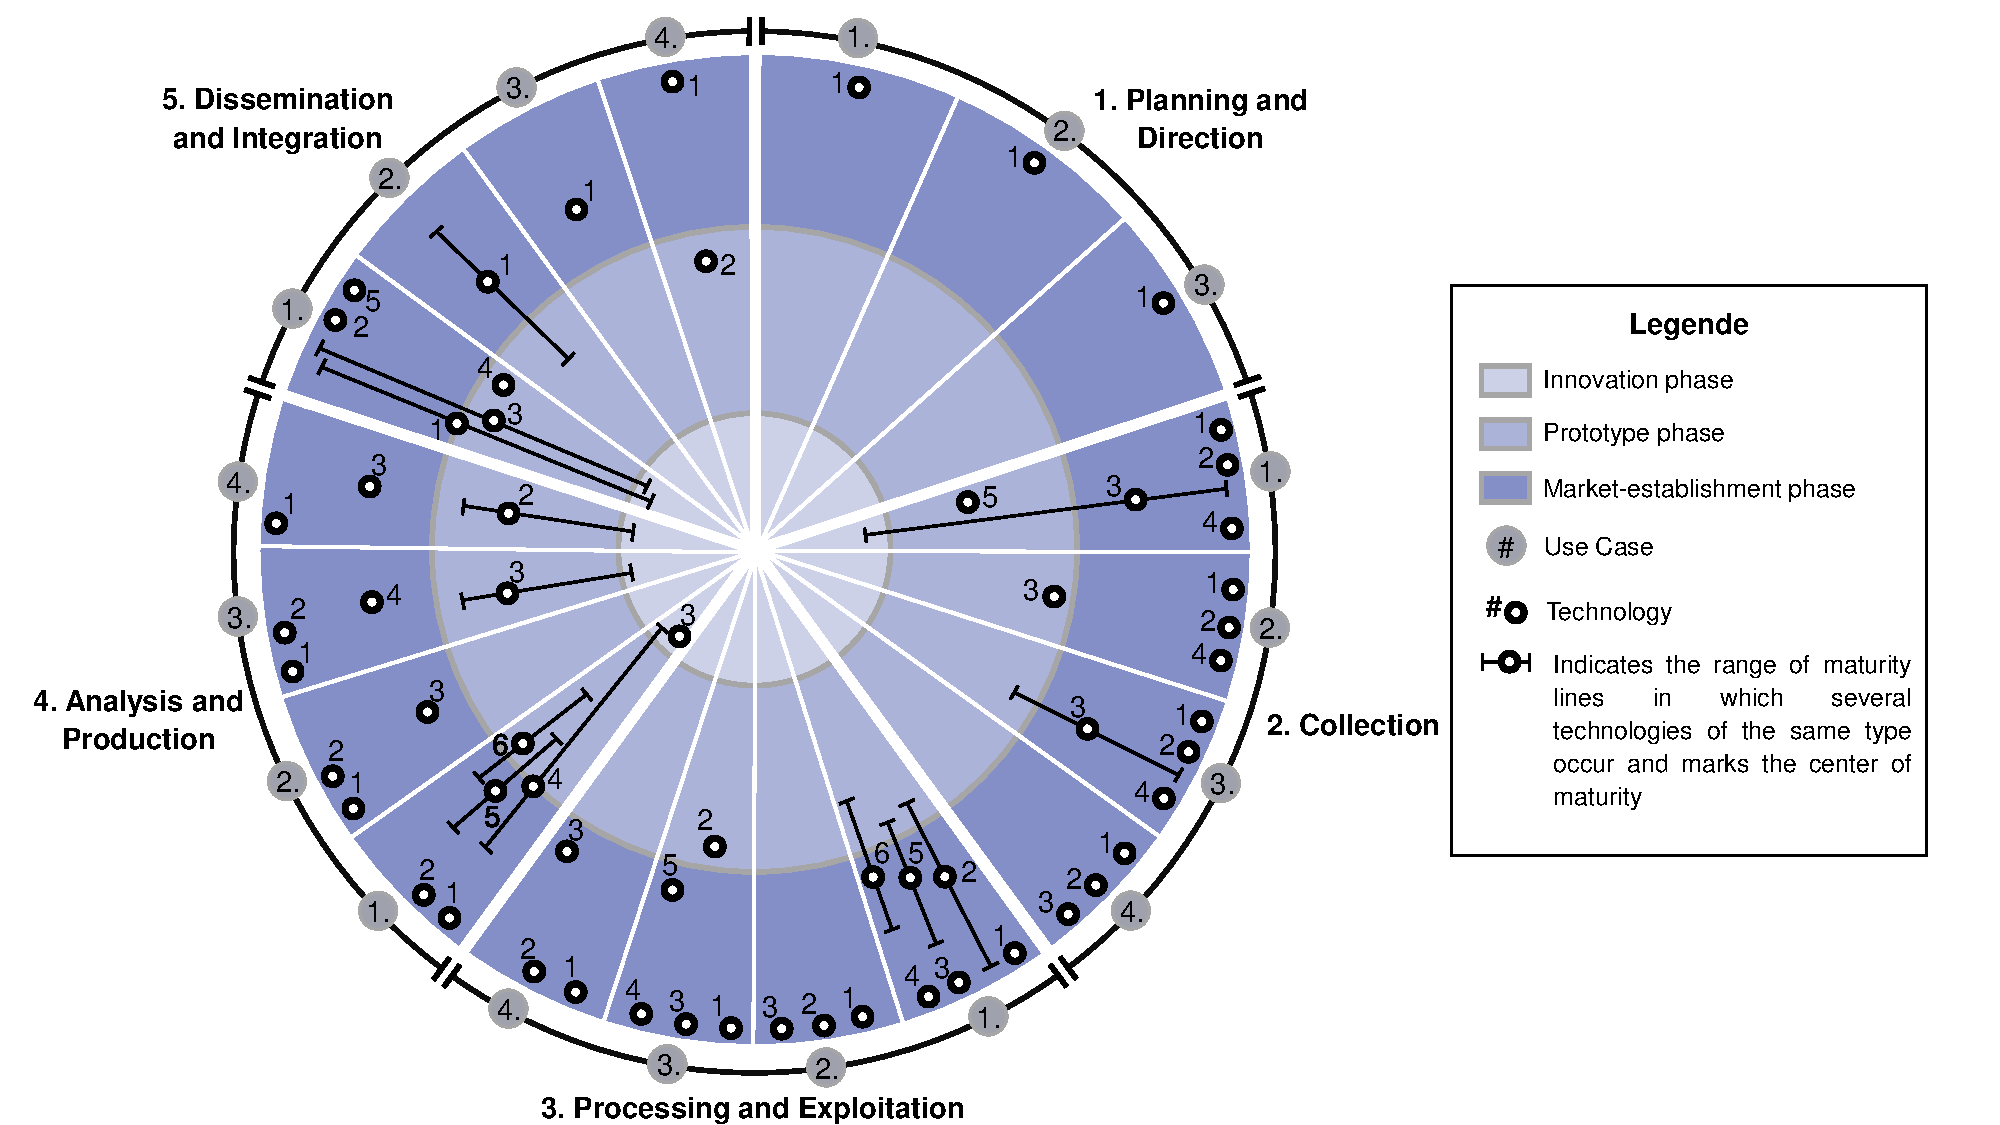
\includegraphics[width=0.8\textwidth]{PDF/images/crop_Trendradar}
    \caption{Trend radar}
    \label{fig:trendradar}
\end{figure*}

\begin{figure*}[!thb]
    \centering
    \rotatebox{90}{%
        \begin{minipage}{\textheight}
            \centering
            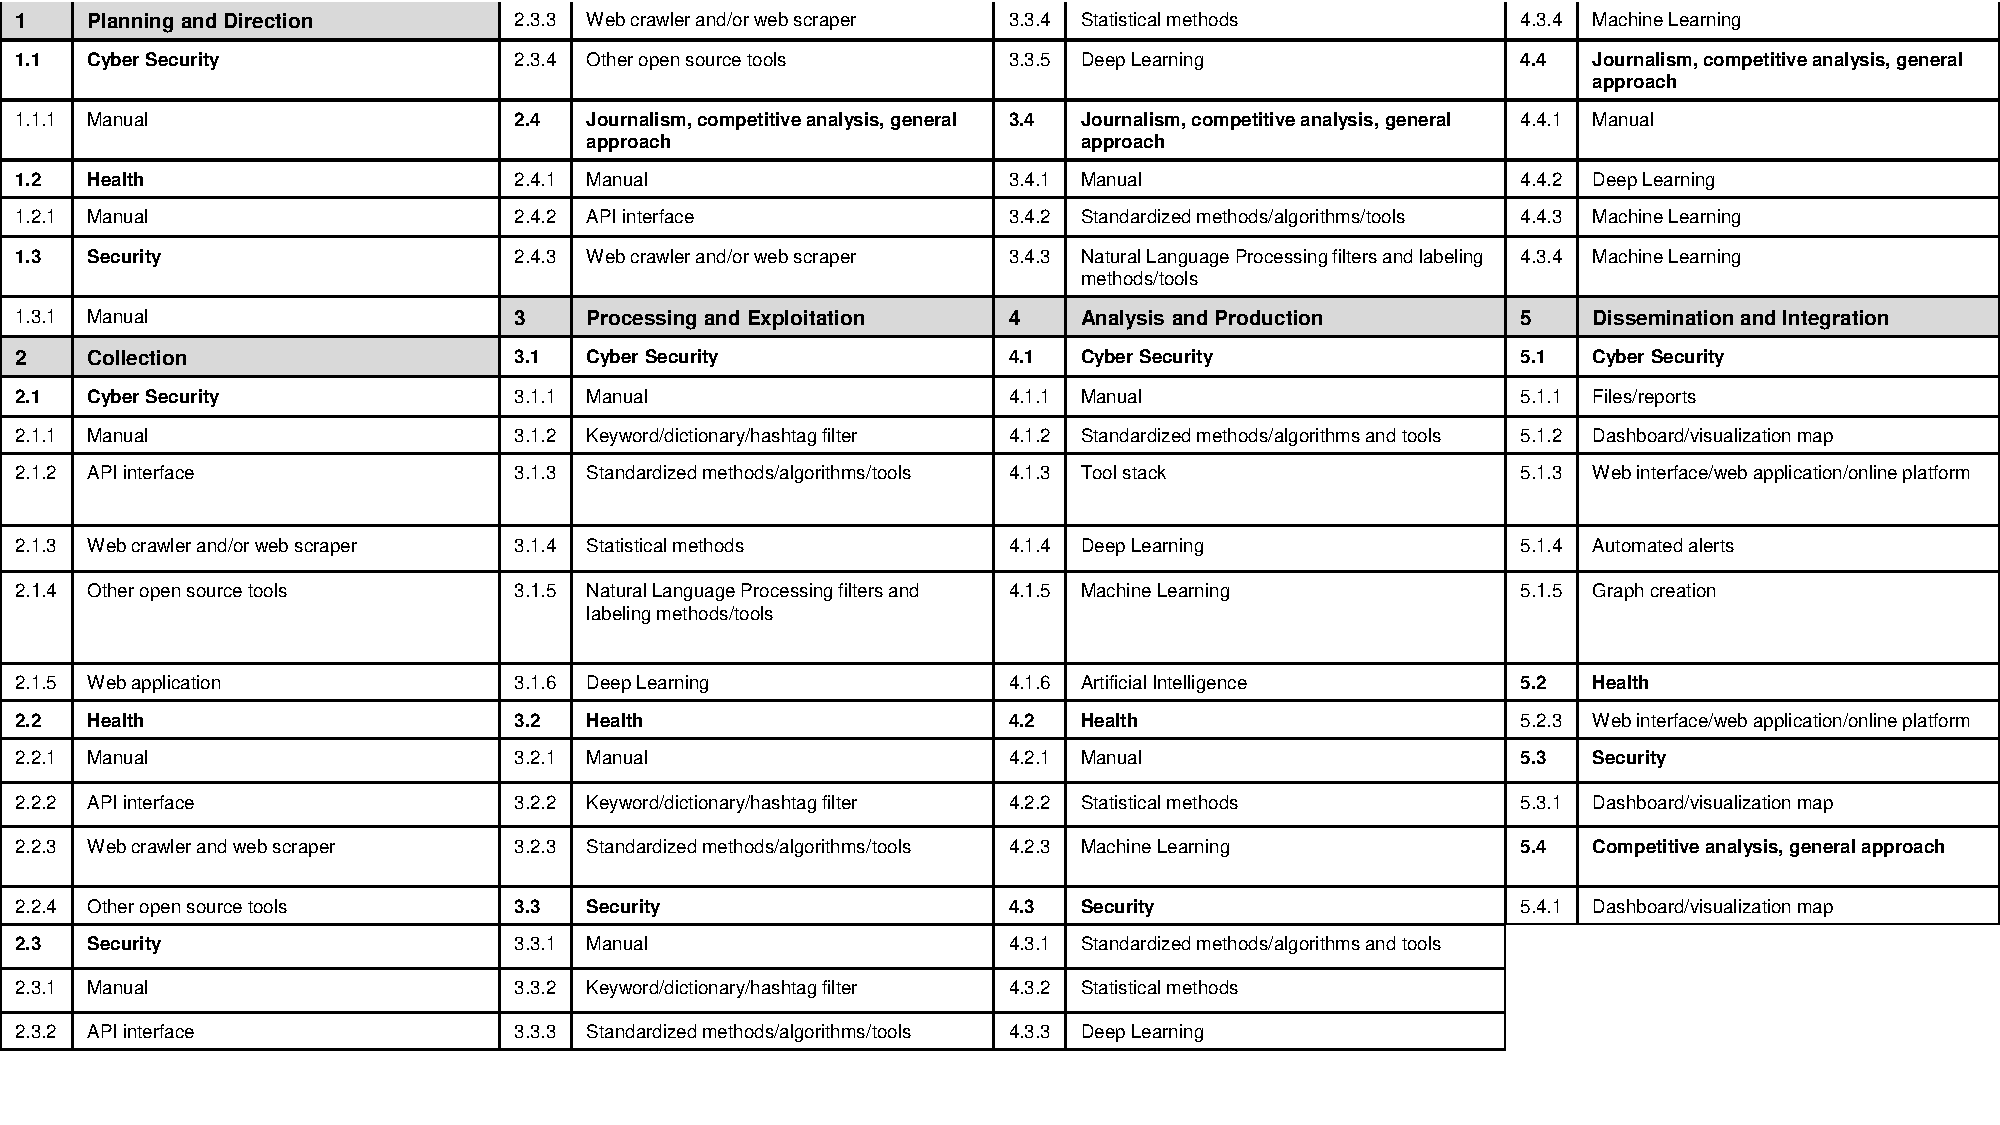
\includegraphics[width=\linewidth]{PDF/images/crop_Trendradar explanation}
            \caption{Trend radar explanation}
            \label{fig:trendradarexplanation}
        \end{minipage}%
    }
\end{figure*}


\subsection{Intelligence Cycle in Theory-Practice Comparison}

Studies could be attributed to each of the Intelligence Cycle phases. However,
none of the applications identified covers all phases in the sense of a third-generation
OSINT tool. Literature primarily focuses on the collection phase, followed by
the analysis and production phase and the processing and exploitation phase.
The dissemination and integration phase is covered by far the least after the planning
and direction phase.

These findings align with the experts' practical experiences. They regard the Intelligence Cycle as "state of the art" (cf. E3, 28.12.2023), but note different manifestations of the phases in praxis (cf. E4, 02.08.2023).
The planning and direction phase is often neglected, despite its crucial importance, leading to wasteful production (cf. E3, 28.07.2023). Conversely, OSINT is frequently associated solely with the collection phase,
resulting in subpar outcomes due to high volumes of low-quality data (cf. E1, 14.07.2023; E2, 19.07.2023; E3, 28.07.2023). The main reason for this is, that the Intelligence Cycle is operated by at least three groups of people. Firstly, the customers, usually located at the "decision-maker level", with a primarily legal professional background (cf. E2, 19.07.2023).
The second is the technician who carries out the data collection and processing (cf. E2, 19.07.2023; E3, 28.07.2023). Lastly, the analyst evaluates the data and creates the intelligence product (cf. E1, 14.07.2023). The process thereby is rarely transparent between the parties
(cf. E1, 14.07.2023; E2, 19.07.2023) and is rarely anchored at the organizational level (cf. E4, 02.08.2023). According to the experts, there is thus no third-generation
OSINT tool in use, at least not in German authorities. In addition, the collection focus is driven by concerns about missing vital information, which could later be revealed as publicly available (cf. E1, 14.07.2023).

\subsection{Use Cases in Theory-Practice Comparison}

Five main use cases emerged from the research: Cyber Security, Health, Security, Journalism,
and Competition Analysis. Cyber Security studies primarily focus on Open Source Cyber Threat
Intelligence (OSCTI), which involves collecting, monitoring, and analyzing publicly available
data to detect potential cyber threats \cite{Ahuja.2022,AlDmour.2023}.
Health applications mainly pertain to COVID-19, such as investigating the epidemic outbreak \cite{Kpozehouen.2020}.
The security use case includes applications such as
analyzing violent behavior in public transport \cite{Nobili.2021}. The identified Journalism study examines the
Twitter activities of the OSINT journalists' association "Bellingcat" \cite{Bar.2023}. Competitive analysis
involves for example the performance classification of Chinese logistics companies \cite{Tao.2023}. Additionally, two
studies could be identified on general approaches to creating knowledge graphs on OSINF \cite{Hu.2023,Ma.2022}.

According to the experts, OSINT is applied in all authorities and has proven itself
in numerous use cases, even if not always explicitly labeled as such (cf. E2, 19.07.2023).
Most common cases are in cyber security/CTI (cf. E1, 14.07.2023; E2, 19.07.2023), as well as general security,
particularly with regard to the German Armed Forces, the (Federal) Intelligence Service,
the German domestic intelligence services and the police.

\subsection{Technologies and Maturity Levels in Theory-Practice Comparison}

Except for the initial phase, automated technologies are utilized across all subsequent phases and use cases.
These technologies demonstrate considerable market maturity, yet manual activities remain prevalent.
The highest level of automation is observed in the CTI use case.

The most advanced automated technologies in the collection phase are web crawlers and/or web scrapers.
Established technologies include "off the shelf" tools (cf. \cite{Middleton.2020}) and open source
solutions like "Tweepy", a Python library for Twitter crawlers (e.g., \cite{Adewopo.2020}).
More advanced prototypes involve combining parallelized, recursive, source-specific web crawlers and scrapers for improved
data collection (e.g.,\cite{Jenkins.2021}). Another method in the prototype phase is
"focused crawling", adapting the crawling path dynamically using a content-driven ML algorithm, BERT ("Bidirectional Encoder Representation from Transformers")
(cf. \cite{Kuehn.2023}). Technologies for crawling/scraping the dark web, like "Torsion" (cf. \cite{Sonawane.2022}),
were assigned to the innovation phase. The experts also note the increasing use of open source tools alongside manual work
(cf. E1, 14.07.2023; E3, 28.07.2023; E1, 14.07.2023). However, they consider traditional web crawling and scraping
outdated due to errors, implementation difficulties, and website resistance. Screenshot-based "web shooting" with
subsequent OCR (Optical Character Recognition) extraction is seen as more modern and robust (cf. E3, 28.07.2023).

NLP applications/methods such as "Topic Classifying," "Part-of-Speech Tagging", "Entity and Relation Annotation", and "Named Entity Recognition"
demonstrate high automation levels in the processing and utilization phase. Technologies commonly used include
the "Python NLTK Toolkit" \cite{Hubbard.2022} and the "Stanford CoreNLP Toolkit" \cite{Middleton.2020}.
Additionally, deep learning, particularly through "word embedding" using the "word2vec" algorithm, is prominent
(e.g., \cite{Bai.2020}). However, the experts note that
this phase within authorities predominantly involves manual work due to the irreplaceable domain knowledge of experts
(cf. E1, 14.07.2023; E2, 19.07.2023; E3, 28.07.2023). The degree of automation of technologies thus depends on the abstraction level.
Operational tasks, which often require specific individual information, show lower automation levels compared to long-term general strategic analyses
requiring extensive data (cf. E3, 28.07.2023).

The highest automation level is observed in the analysis and production phase, where AI, ML, and DL technologies are prevalent.
Under DL, vectorization algorithms can also be found. Particularly BERT algorithms in different versions are commonly utilized
(e.g., \cite{Ma.2022}). Furthermore, even under ML vectorization models such as BERT or
"Supervised Support Vector Machines" (SVM) (e.g., \cite{Iorga.2020}) are listed.
In addition, the algorithms "Random Forest", XGBoost ("eXtreme Gradient Boosting)",
lightGBM ("light Gradient Boosting Machine"), "Naive Bayes" and "logistic regressions" are particularly common.
Publications thereby often utilize multiple algorithms concurrently for performance comparison (e.g. \cite{Tao.2023})
or for layered analysis (e.g. \cite{Yang.2022}). AI technologies are generally less specified,
except for \cite{Dale.2023}, who developed a bidirectional recurrent neural network with
BiGur ("Bidirectional Gated Recurrent Unit") layers. Due to the modular use of publicly available models,
the technologies are mostly classified as market-ready. Despite the potential, practical work in this phase
largely relies on manual content analysis due to a lack of technological understanding and acceptance,
especially at the contractor/provider level in Germany (cf. E2, 19.07.2023; E3, 28.07.2023; E4, 02.08.2023). Furthermore,
ethical and legal barriers, such as GDPR (General Data Protection Regulation), hinder technology adoption
(cf. E2, 19.07.2023; E4, 02.08.2023). Additionally, security concerns in German authorities favor
standalone systems (cf. E2, 19.07.2023). If smart technologies are used, it is often only inofficially
(cf. E4, 02.08.2023). However, there's a need for modular, dynamically expandable
systems to keep pace with rapid advancements (cf. E1, 14.07.2023; E3, 28.07.2023; E4, 02.08.2023).
Nevertheless, human experience and specialization should not be outweighed, but rather a certain product quality
be ensured in a supportive manner. Yet, the revolutionary potential of large language models (LLM) cannot be estimated (cf. E4, 02.08.2023).

In the dissemination and integration phase, tools like "Power BI" \cite{Tao.2023}
are utilized to create dashboards and visualization maps. Furthermore, user interfaces,
web applications, and online platforms are developed, including Python GUIs,
specific browser applications \cite{Elmas.2022},
improved user interfaces and input masks for entire tool stacks \cite{Arjun.2020}.
Additionally, Technologies for generating automated alerts, particularly for cyber security risk assessments,
are prevalent \cite{Ahuja.2022}. Graph-based visualizations are also common, utilizing tools
/libraries like "Matplot," "Networkx," "Pygraphistry," or the "Neo4j-Browser" \cite{Middleton.2020}.
Except from the alerts, the retrieval of results is largely semi-automated and the technologies are in the
market establishment phase. No information on targeted user tests or a new development run involving
user feedback could thereby be found in any of the studies. The experts state that there is still very little
automation within the authorities during this phase. The final product is often only a PDF document,
an email or a verbal report (cf. E1, 14.07.2023), although in many cases no more is required (cf. E3, 28.07.2023).
However, outside of the OSINT topic, there are several automated tools, that could be transferred
to the authorities in this context (cf. E4 02.08.2023). Moreover, in practice, there is also a lack of
necessary feedback for product improvement (cf. E3, 28.07.2023).

\section{Discussion and Conclusion} \label{sec:discussion}
%\section{Discussion} \label{sec:discussion}
\subsection{Contributions and Implications}

The investigation into the existence of a robust, automated third-generation OSINT system
(e.g., \cite{Ghioni.2023})
leads to a negative conclusion, at least for Germany. Identified applications fall short of fully covering
the intelligence cycle, with significant gaps in the planning and direction phase,
followed by the dissemination and integration phase. Humans therefore remain the driving (analysis)
component. However, the finding by Pastor-Galindo et al. \cite{PastorGalindo.2020} that intelligent OSINT
concepts are not yet widespread cannot be confirmed either. Numerous intelligent tools available
on the market were identified in the other phases. Nevertheless, practical integration has so far
fallen short of the (theoretical) possibilities. Yet this finding likewise does not confirm the
thesis of Yogish et al. \cite{Yogish.2021} that automated, AI-driven solutions, largely eliminating
the human component, are inevitably required in every area of OSINT. Rather, the key research
question should be why proven, available applications whose support is needed have not
yet found widespread use, especially in intelligence authorities. In addition, the question of how the
first and last Intelligent Cycle phases, alongside the others, can be better supported technically
should be investigated.

Addressing these research questions entails resolving numerous underlying research gaps (RGs), directly corresponding to the three key groups involved in the intelligence cycle.

%\begin{itemize}
%    \item[\textbf{RG1:}] \textbf{Deficiency in Initial Phase Tools:} There is a technological gap in tools that cover the initial phase of the intelligence cycle, particularly in frameworks for targeted requirements definition and communication. This gap contributes to an overemphasis on the collection phase \cite{Lowenthal.2020}.
%
%    \item[\textbf{RG2:}] \textbf{Lack of Dissemination Mechanisms:} There is a dearth of effective dissemination and integration mechanisms tailored for authorities, largely due to insufficient user testing and iterative feedback incorporation. The indispensability of consumer feedback is underscored by established frameworks to enhance product quality and reduce data overload \cite{DirectorofNationalIntelligence.2011,JointChiefsofStaffU.S.Army.2013,NorthAtlanticTreatyOrganization.2001,Gibson.2016,Day.2016}.
%
%    \item[\textbf{RG3:}] \textbf{Modular OSINT Systems:} The future of OSINT systems hinges on modular concepts, yet only limited research has been conducted in this area \cite{Arjun.2020,Wright.2020}.
%
%    \item[\textbf{RG4:}] \textbf{Revamping Procurement Procedures:} It's crucial to move away from monolithic stand-alone setups in procurement procedures.
%
%    \item[\textbf{RG5:}] \textbf{Ethical and Legal Compliance:} Ensuring compliance with ethical and legal principles is vital for product adoption, requiring robust legislative updates and considering both national and international regulations, such as GDPR \cite{EuropeanParliament.2016,EuropeanCommission.18.08.2023,Ghioni.2023,Wittmer.2022}.
%
%    \item[\textbf{RG6:}] \textbf{Technical Understanding among Decision Makers:} Addressing challenges necessitates foundational technical understanding at decision-maker levels, fostering openness to technology and cultivating an information-sharing mindset to transcend bureaucratic barriers \cite{NorthAtlanticTreatyOrganization.2001}.
%
%    \item[\textbf{RG7:}] \textbf{Use of LLMs in Intelligence:} While Large Language Models (LLMs) show promise in intelligence analysis, their application in operational settings is underexplored \cite{Radford.2023,Zhao.31.03.2023}.
%
%    \item[\textbf{RG8:}] \textbf{Technological Tools for Technicians:} Technicians often handle significant phases of the intelligence cycle independently, yet there is a notable absence of robust collection tools to match the rapidly evolving media landscape.
%
%    \item[\textbf{RG9:}] \textbf{Coordination between Analysts and Technicians:} Coordination gaps between analysts and technicians pose risks of excessive data collection, emphasizing the need for tools that enhance transparency and mitigate collection biases \cite{Lowenthal.2020}.
%\end{itemize}

\textbf{RG1 - Deficiency in Initial Phase Tools:} There is a technological gap in tools that cover the initial phase of the intelligence cycle, particularly in frameworks for targeted requirements definition and communication.
%This gap contributes to an overemphasis on the collection phase \cite{Lowenthal.2020}.

\textbf{RG2 - Lack of Dissemination Mechanisms:} There is a dearth of effective dissemination and integration mechanisms tailored for authorities, largely due to insufficient user testing and iterative feedback incorporation. The indispensability of consumer feedback is underscored by established frameworks to enhance product quality and reduce data overload \cite{DirectorofNationalIntelligence.2011,JointChiefsofStaffU.S.Army.2013,NorthAtlanticTreatyOrganization.2001,Gibson.2016,Day.2016}.

\textbf{RG3 - Modular OSINT Systems:} The future of OSINT systems hinges on modular concepts, yet only limited research has been conducted in this area \cite{Arjun.2020,Wright.2020}.

\textbf{RG4 - Revamping Procurement Procedures:} It's crucial to move away from monolithic stand-alone setups in procurement procedures.

\textbf{RG5 - Ethical and Legal Compliance:} Ensuring compliance with ethical and legal principles is vital for product adoption, requiring robust legislative updates and considering both national and international regulations, such as GDPR \cite{EuropeanParliament.2016,EuropeanCommission.18.08.2023,Ghioni.2023}.

\textbf{RG6 - Technical Understanding among Decision Makers:} Addressing challenges necessitates foundational technical understanding at decision-maker levels, fostering openness to technology and cultivating an information-sharing mindset to transcend bureaucratic barriers \cite{NorthAtlanticTreatyOrganization.2001}.

\textbf{RG7 - Use of LLMs in Intelligence:} While Large Language Models (LLMs) show promise in intelligence analysis, their application in operational settings is underexplored \cite{Radford.2023,Zhao.31.03.2023}.

\textbf{RG8 - Technological Tools for Technicians:} Technicians often handle significant phases of the intelligence cycle independently, yet there is a notable absence of robust collection tools to match the rapidly evolving media landscape.

\textbf{RG9 - Coordination between Analysts and Technicians:} Coordination gaps between analysts and technicians pose risks of excessive data collection, emphasizing the need for tools that enhance transparency and mitigate collection biases \cite{Lowenthal.2020}.

%These gaps highlight the critical areas for future development and research to enhance the efficiency and effectiveness of intelligence operations.

\subsection{Limitations and Future Research}

The first limitation relates to the fact that, due to a lack of clarity about the legal
and ethical basis \cite{Ghioni.2023,Wittmer.2022},
it could not be verified whether only public sources \cite{NorthAtlanticTreatyOrganization.2002} were used
in the analyzed studies. It was also not verified whether the technologies meet the
legal and ethical requirements for the use of the information obtained
\cite{PastorGalindo.2020,Wittmer.2022}. The second
limitation stems from classification categories not fully aligning with the
MECE (Mutually-Exclusive-and-Collectively-Exhaustive) principle \cite{Lee.2018},
particularly evident in the hierarchical dependency of AI, ML, and DL technologies. In addition,
the wording of the authors was followed for objective reproduction when identifying the technologies,
but the accuracy of the information was not reviewed in detail. Moreover, no fixed limits could be defined
for the volume category, as these were not recorded in uniform dimensions in the studies.
The third limitation concerns the limited sample size in expert interviews. Due to the
extremely difficult-to-access target group, the active user level and the decision-maker
level within the authorities were not interviewed. For improved intercoder reliability,
independent verification of the coding carried out by at least a second researcher
is also recommended \cite{Bogner.2002c,Glaser.2009}.
Lastly, the research structure, following the DSRM process, was executed linearly rather
than iteratively as recommended \cite{Peffers.2007}.

Nevertheless, the study furnishes future researchers with a comprehensive knowledge base on OSINT
through a practice-validated trend radar.
%The radar serves as a comprehensive knowledge base, allowing for contemporary evaluation and analysis of OSINT technologies.
Initial evaluations reveal two crucial unanswered research questions and identifies nine detailed research gaps, highlighting
critical areas for future development and research to enhance the efficiency and effectiveness of intelligence operations.
%as well as identifying research gaps for future studies, penetrating the complex research field. 
Moreover, the developed trend radar serves as a guideline for practitioners. The radar
is adaptable to the evolving subject area and transferable to other intelligence disciplines.


%Before addressing these questions, future researchers are advised to validate them further. 
%Utilizing the presented tools to reevaluate literature
%categorization and update identified technologies is recommended. In addition, semantic
%control and indexing methods (e.g. LLM) should be included. Due to the high dynamic of the research field,
%it is also recommended to integrate news articles and scientific journals with shorter publication cycles.
%Reassessing categories based on MECE criteria and conducting further interviews, including internationally
%and with active authority members, is advisable. Employing methods like the Delphi technique to evaluate
%trends and establish consensus is suggested \cite{Hader.2000}. Subsequent iterations of the design process and adjustments
%to the trend radar, if necessary, should follow based on these results \cite{Peffers.2007,Sonnenberg.2012}.

%\subsection{Conclusion}
%\subsection{Summary}

%In this paper, a practice-validated trend radar was developed that depicts current trends
%in the field of OSINT through applied technologies. It serves as a comprehensive knowledge base,
%allowing for contemporary evaluation and analysis of OSINT technologies as well as identifying research
%gaps for future studies, penetrating the complex research field. Moreover, it serves as a guideline for practitioners. The radar
%is adaptable to the evolving subject area and transferable to other intelligence disciplines.
%Based on the developed trend radar, current research gaps are identified and new research questions are raised.

%Results reveal the absence of an automated third-generation OSINT system in Germany, highlighting the
%need for technological support in the planning and direction as well as the dissemination and integration phases.
%The research questions identified for future studies are therefore, why proven, available applications,
%have not yet found widespread use, especially in the security authorities.
%In addition, the question of how the first and last Intelligent Cycle phases, alongside the others,
%can be better supported technically is to be investigated. The research gaps identified extend
%not only to technology but in particular to the legal, administrative, political and
%social sciences, necessitating interdisciplinary collaboration. Above all, a need to catch up is seen
%in the non-technical research fields, responsible for creating the decisive prerequisites for technology
%implementation.


% Fonts specification --- not shown as it doesn't exist in the Word document either. 

%\section{Fonts}

%A summary of fonts is provided in Table \ref{tab: fonts}. 

%\begin{table}[thb]
%\centering
%\caption{\label{font-table} Font guide. \vskip 3pt }
%\label{tab: fonts}
%\begin{tabular}{l|rl}
%\hline \bf Type of Text & \bf Font Size & \bf Style \\ \hline
%paper title & 14 pt &  \bf bold \\
%authors & 10 pt &  \underline{email} underlined \\
%abstract title & 12 pt &  \bf bold\\
%abstract text & 10 pt &  \it italic\\
%section titles & 12 pt & \bf bold \\
%subsection titles & 11 pt & \bf bold \\
%document text & 10 pt  & \\
%captions & 9 pt & \sansserifformat{\captionsize sans-serif, \bf bold} \\
%bibliography & 9 pt & \\
%footnotes & 8 pt & \\
%\hline
%\end{tabular}
%\end{table}


\section{References}


%Bibliography 

\bibliographystyle{ieeetr}
\bibliography{references}

\end{document}
